\documentclass[]{article}
\usepackage{pgf-umlcd}
%\usepackage{tikzsymbols}
\usepackage[a4paper,landscape, margin={3cm}]{geometry}


%opening
\title{}
\author{}

\begin{document}
	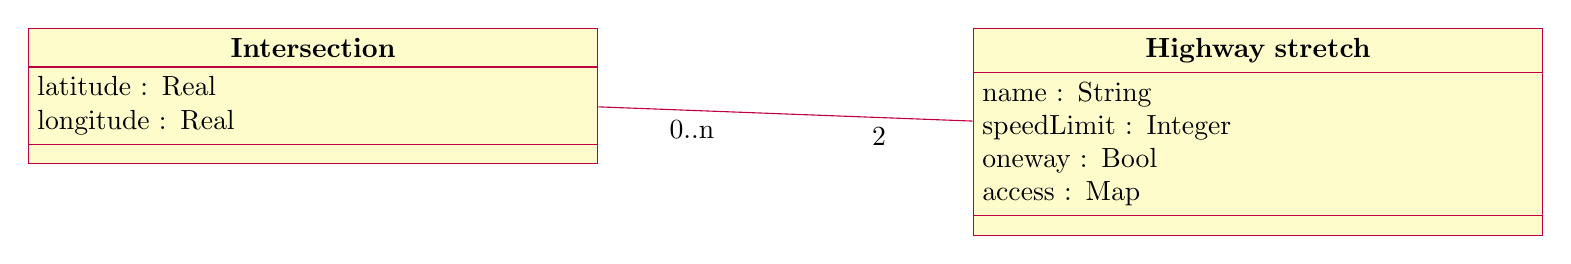
\begin{tikzpicture}
		\begin{class}[text width=7cm]{Intersection}{0,0}
			\attribute{latitude : Real}
			\attribute{longitude : Real}	
		\end{class}
	
		\begin{class}[text width=7cm]{Highway stretch}{12,0}
			\attribute{name : String}
			\attribute{speedLimit : Integer}
			\attribute{oneway : Bool}
			\attribute{access : Map}
		\end{class}
		
		%%% RELAZIONI
		\association
			{Intersection}{}{0..n}
			{Highway stretch}{}{2}
	\end{tikzpicture}
\end{document}
